% ==================================================================
% Post-hoc trajectory optimization + the attempt to learn it
% (gated tail adapter).
% FRAMES ONLY -- \input this into main.tex (preamble lives there).
%
% Needs: beamer, amsmath, amssymb, booktabs, graphicx, tikz.
% Figures: figs/posthoc_fix_*.png (put figs/ on \graphicspath).
% The figures are cropped here with trim/clip; trims are in bp for
% the 110-dpi PNGs written by tools/plot_fix_pairs.py.
% ==================================================================
\usetikzlibrary{arrows.meta,positioning,calc}

% ---- colors (namespaced) -----------------------------------------
\definecolor{phBase}{HTML}{6B7280}
\definecolor{phOpt}{HTML}{2A7BDE}
\definecolor{phEdge}{HTML}{2A303A}
\definecolor{phDrive}{HTML}{E9ECF1}
\definecolor{phBaseSoft}{HTML}{D7DAE0}
\definecolor{phOptSoft}{HTML}{CFE2F8}
\definecolor{phFrozen}{HTML}{EEF0F3}
\definecolor{phGood}{HTML}{0C8571}
\definecolor{phBad}{HTML}{CE4325}
\newcommand{\phgood}[1]{\textcolor{phGood}{#1}}
\newcommand{\phbad}[1]{\textcolor{phBad}{#1}}

% ---- headline numbers (term-aware, 1450 held-out scenes x 4 seeds) --
% o_am, select/lateral_opt_argmin_20261002_142129_3029435, select_summary_term.json
\newcommand{\phBaseF}{0.306}  \newcommand{\phOptF}{0.903}
\newcommand{\phBaseI}{0.545}  \newcommand{\phOptI}{0.956}
\newcommand{\phBaseS}{0.9975} \newcommand{\phOptS}{0.9992}
\newcommand{\phBaseM}{0.9739} \newcommand{\phOptM}{0.9965}
\newcommand{\phOptD}{+0.0227} \newcommand{\phOptCI}{[+0.020,\,+0.025]}


% ##################################################################
\section{Post-hoc trajectory optimization}
% ##################################################################

% ------------------------------------------------------------------
\begin{frame}{Post-hoc optimization: edit the plan the policy already made}
  \begin{itemize}\itemsep6pt
    \item At every replan the \textbf{frozen} diffusion policy samples a plan.
    \item We edit only its next 2\,s, with two numbers per step:
          \begin{itemize}\itemsep2pt
            \item $d_t$: shift \textbf{sideways} (perpendicular to the route)
            \item $s_t$: shift \textbf{along} the route (faster / slower)
          \end{itemize}
    \item Pick $(d,s)$ by minimizing one loss: \quad $L = \text{Safety} + \text{Comfort}$
    \item Execute the edited plan. \textbf{No trigger, no acceptance test:}
          a plan already clear of every margin has $L=0$ with no edit, so it
          runs unchanged.
    \item No training --- the pretrained policy is used as is.
  \end{itemize}
\end{frame}

% ------------------------------------------------------------------
\begin{frame}{Results: the failures are fixed, the successes are kept}
  \small
  \begin{center}
  \begin{tabular}{@{}lcccc@{}}
    \toprule
    solved rate & failure & intermittent & success & \textbf{marginal} \\
    \midrule
    base policy             & \phBaseF & \phBaseI & \phBaseS & \phBaseM \\
    \footnotesize\quad collided & \footnotesize 0.198 & \footnotesize 0.131 & \footnotesize 0.0005 & \\
    \footnotesize\quad off-road & \footnotesize 0.487 & \footnotesize 0.325 & \footnotesize 0.0020 & \\
    \footnotesize\quad no goal  & \footnotesize 0.009 & \footnotesize 0.000 & \footnotesize 0.0000 & \\
    \midrule
    + post-hoc optimization & \textbf{\phOptF} & \textbf{\phOptI} & \textbf{\phOptS}
                            & \textbf{\phOptM}~(\phgood{\phOptD}) \\
    \footnotesize\quad collided & \footnotesize 0.040 & \footnotesize 0.024 & \footnotesize 0.0008 & \\
    \footnotesize\quad off-road & \footnotesize 0.038 & \footnotesize 0.018 & \footnotesize 0.0000 & \\
    \footnotesize\quad no goal  & \footnotesize 0.019 & \footnotesize 0.002 & \footnotesize 0.0000 & \\
    \bottomrule
  \end{tabular}
  \end{center}
  \begin{itemize}\itemsep2pt
    \item \textbf{Splits} come from running the base policy with 4 seeds per scene:
          \textbf{success} = solved all 4, \textbf{failure} = solved none,
          \textbf{intermittent} = solved some but not all.
          Held-out: 173 / 277 / 1000 scenes, each re-run with 4 seeds.
    \item \textbf{Solved} = reaches the goal, never off-road, never collides.
          Unsolved episodes split into collided (any collision), off-road
          (without a collision), and no goal (clean, but never arrives).
    \item \textbf{Marginal} = corpus-level solved rate: the splits re-weighted to
          their share of the corpus (failure 1.5\%, intermittent 3.0\%,
          success 95.6\%). 95\% CI of the gain: \phOptCI.
  \end{itemize}
  \vspace{2pt}
  \footnotesize\textcolor{gray}{Why the base solves 0.31 of ``failures'': the splits
  were built before a bug fix. The planner read its time step from the first
  timestamp pair ($\approx$0.075\,s instead of 0.1\,s) in some scenes, so plans
  ran at $\approx$0.75$\times$ speed and never reached the goal. After the fix the
  base solves those scenes (44 of the 173) $\sim$95\% of the time.}
\end{frame}

% ------------------------------------------------------------------
% Crops: row 1 = whole episode, row 2 = zoom; titles and caption removed.
\newcommand{\phrowA}[1]{\includegraphics[height=2.6cm,trim=36 367 39 64,clip]{#1}}
\newcommand{\phrowB}[1]{\includegraphics[height=2.6cm,trim=36 21 39 411,clip]{#1}}
\newcommand{\phlabels}{%
  \makebox[2.87cm]{\scriptsize\textcolor{phBase}{\textbf{base policy}}}%
  \makebox[2.87cm]{\scriptsize\textcolor{phOpt}{\textbf{optimized}}}}

\begin{frame}{Before / after}
  \begin{columns}[T]
    \column{0.49\textwidth}
    \centering
    {\scriptsize scene 33174: base goes off-road $\to$ solved}\\[1pt]
    \phlabels\\
    \phrowA{posthoc_fix_33174}\\[2pt]
    \phrowB{posthoc_fix_33174}

    \column{0.49\textwidth}
    \centering
    {\scriptsize scene 59208: base goes off-road $\to$ solved}\\[1pt]
    \phlabels\\
    \phrowA{posthoc_fix_59208}\\[2pt]
    \phrowB{posthoc_fix_59208}
  \end{columns}
  \vspace{3pt}
  {\scriptsize Top: whole episode. Bottom: zoom at the closest approach to a road
  edge; \textcolor{phBase}{dashed} = the policy's plan the optimizer replaced.
  Black = road edge, grey = lanes / other cars, star = goal.}
\end{frame}

% ------------------------------------------------------------------
\begin{frame}{How it's done (1/2): the edit and the safety loss}
  \small
  \begin{columns}[T]
    \column{0.5\textwidth}
    \textbf{Edit} ($n{=}20$ steps of $0.1$\,s):
    \[ p'_t = \mathrm{route}(S_t + s_t) + d_t\,\mathbf{n}_t \]
    {\footnotesize $S_t$: how far along its route the plan is at step $t$;
    $\mathbf{n}_t$: the car's left direction. Heading and speed are
    recomputed from $p'$.}

    \medskip
    \textbf{Safety}:
    \[ \mathrm{Safety} = \tfrac1n \sum_t \Big[\sum_{k=1}^{4} B_e\big(c^{e}_{t,k}\big)
                + \sum_j B_a\big(c^{a}_{t,j}\big)\Big] \]
    \begin{itemize}\itemsep1pt\footnotesize
      \item $c^{e}_{t,k}$: distance of car corner $k$ to the road edge ($<0$ = off-road)
      \item $c^{a}_{t,j}$: gap to car $j$ ($<0$ = collision); other cars
            predicted at \textbf{constant velocity}
    \end{itemize}

    \column{0.5\textwidth}
    \textbf{Barrier} $B$: a smoothed hinge (margin $m$, knee width $\tau$)
    \[ B(c) = \begin{cases}
         0 & c \ge m \\[2pt]
         \dfrac{(m-c)^2}{2\tau} & m-\tau < c < m \\[6pt]
         (m-c) - \tfrac{\tau}{2} & c \le m-\tau
       \end{cases} \]
    \begin{itemize}\itemsep1pt\footnotesize
      \item $B_e$ (road edge): $m{=}0.3$\,m, $\tau{=}0.15$\,m;
            $B_a$ (other cars): $m{=}0.75$\,m, $\tau{=}0.25$\,m.
            Margins = human drivers' 1st-percentile clearance.
      \item Clear of the margin: \textbf{exactly zero}, no push.
            Inside: a soft knee, then a constant push.
    \end{itemize}
  \end{columns}
\end{frame}

% ------------------------------------------------------------------
\begin{frame}{How it's done (2/2): comfort and the optimizer}
  \small
  \[ L(d,s) = \mathrm{Safety}(d,s) + C_{\text{lat}}(d) + C_{\text{lon}}(s) \]
  \begin{columns}[T]
    \column{0.5\textwidth}
    \textbf{Comfort} (charged on the \emph{edit}, not the plan):
    \[ C_{\text{lat}} = \tfrac1n\sum_t \Big[\,w_a\,(\ddot d_t)^2 + w_j\,(\dddot d_t)^2\,\Big] \]
    {\footnotesize sideways acceleration + jerk: swerve gently.}
    \[ C_{\text{lon}} = \tfrac1n\sum_t \Big[\,w_a\,(\ddot s_t)^2 + w_j\,(\dddot s_t)^2 + w_p\, s_t^{2}\,\Big] \]
    {\footnotesize braking / speeding up + its jerk + stay on the policy's timing.}

    \column{0.5\textwidth}
    \textbf{Optimizer}: CHOMP --- gradient descent preconditioned by the
    comfort matrix $H$, where $C_{\text{lat}} + C_{\text{lon}} = \tfrac12 x^\top H x$:
    \[ x \leftarrow x - \eta\,H^{-1}\nabla L, \qquad x = (d, s) \]
    \begin{itemize}\itemsep1pt\footnotesize
      \item $H^{-1}$ turns a local push (one corner near the edge) into a smooth swerve.
      \item 32 iterations, trust region; start from no edit.
    \end{itemize}
  \end{columns}
\end{frame}


% ##################################################################
\section{Learning the repair}
% ##################################################################

% ------------------------------------------------------------------
\begin{frame}{Learning it: a gated adapter on the frozen UNet}
  \small
  Goal: the policy produces the optimized plan in its own sampling pass ---
  no optimizer at deployment.
  \begin{center}
  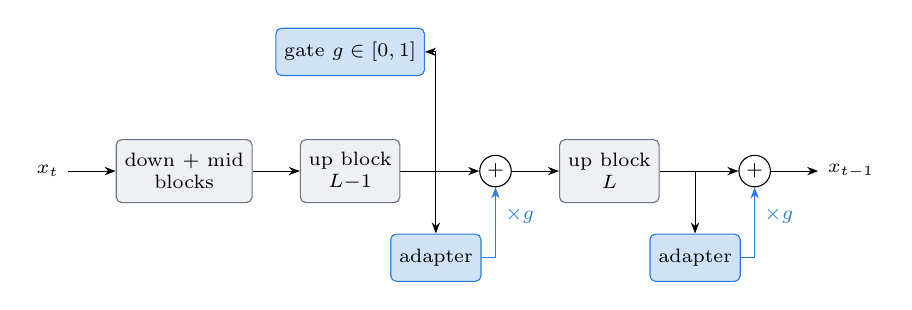
\begin{tikzpicture}[font=\scriptsize,>={Stealth[length=4pt]},node distance=4mm and 6mm,
      blk/.style={draw=phBase,fill=phFrozen,rounded corners=2pt,minimum height=8mm,align=center,inner sep=3pt},
      ada/.style={draw=phOpt,fill=phOptSoft,rounded corners=2pt,minimum height=6mm,align=center,inner sep=3pt},
      sum/.style={circle,draw,inner sep=0pt,minimum size=4mm}]
    \node (in) {$x_t$};
    \node[blk,right=of in] (dm) {down + mid\\blocks};
    \node[blk,right=of dm] (u1) {up block\\$L{-}1$};
    \node[sum,right=10mm of u1] (s1) {$+$};
    \node[blk,right=of s1] (u2) {up block\\$L$};
    \node[sum,right=10mm of u2] (s2) {$+$};
    \node[right=of s2] (out) {$x_{t-1}$};
    \draw[->] (in) -- (dm);  \draw[->] (dm) -- (u1); \draw[->] (u1) -- (s1);
    \draw[->] (s1) -- (u2);  \draw[->] (u2) -- (s2); \draw[->] (s2) -- (out);
    \coordinate (b1) at ($(u1.east)!0.45!(s1.west)$);
    \coordinate (b2) at ($(u2.east)!0.45!(s2.west)$);
    \node[ada] (a1) at ([yshift=-11mm]b1) {adapter};
    \node[ada] (a2) at ([yshift=-11mm]b2) {adapter};
    \draw[->] (b1) -- (a1); \draw[->,phOpt] (a1) -| node[pos=0.8,right] {$\times g$} (s1);
    \draw[->] (b2) -- (a2); \draw[->,phOpt] (a2) -| node[pos=0.8,right] {$\times g$} (s2);
    \node[ada,above=8mm of u1] (g) {gate $g\in[0,1]$};
    \draw[->] (b1) |- (g.east);
  \end{tikzpicture}
  \end{center}
  \begin{itemize}\itemsep2pt
    \item Base UNet \textbf{frozen} (grey). Two small residual MLPs after the last two
          up blocks: $h \leftarrow h + g\cdot A(h)$, $A$ zero-initialized, so training
          starts exactly at the base policy.
    \item Gate $g$: one number per sampled plan --- ``does this draw need fixing?''
    \item Active only in the last 5 of 100 denoising steps; 42k new parameters
          (base: 31.7M).
    \item Trained on pairs (this exact base draw, the optimizer's edit of it),
          replayed with the same noise.
  \end{itemize}
\end{frame}

% ------------------------------------------------------------------
\begin{frame}{Learning it: converges on training data, not on held-out}
  \small
  \begin{columns}[T]
    \column{0.44\textwidth}
    \textbf{Offline}: fraction of the base$\to$teacher gap closed
    \begin{center}
    \begin{tabular}{@{}lc@{}}
      \toprule
      64 training repairs & \phgood{0.98--0.99} \\
      held-out repairs     & \phbad{$-0.5$} \\
      \bottomrule
    \end{tabular}
    \end{center}
    {\footnotesize 1 = reproduces the teacher, 0 = no change, $<0$ = moves the
    wrong way. Training repairs are fit to 1--2\,cm; on new scenes the adapter
    does \emph{worse} than no adapter. With the full set (1{,}120 repairs,
    140 scenes) held-out stays at $\approx$0.1.}

    \column{0.56\textwidth}
    \textbf{Closed loop} (held-out, 4 seeds)
    \begin{center}
    \begin{tabular}{@{}lcccc@{}}
      \toprule
      & fail. & interm. & succ. & marg.\ $\Delta$ \\
      \midrule
      base         & 0.306 & 0.538 & 0.9975 & --- \\
      teacher      & 0.903 & 0.951 & 1.0000 & \phgood{$+0.0234$} \\
      adapter, $g{=}1$ & 0.400 & 0.550 & 0.9607 & \phbad{$-0.0334$} \\
      adapter, learned $g$ & 0.366 & 0.547 & 0.9962 & $-0.0001$ \\
      \bottomrule
    \end{tabular}
    \end{center}
    {\footnotesize Always on, it breaks successes; gated, it ties the base.}
  \end{columns}
  \vspace{6pt}
  \begin{alertblock}{Reading}
    The adapter can \emph{represent} a repair but does not learn \emph{how} to repair:
    more capacity (5$\to$10 adapted steps, 4$\times$ wider) does not help on
    held-out scenes. That points to too little repair data, not the architecture.
  \end{alertblock}
\end{frame}
